\documentclass{article}

\usepackage[utf8]{inputenc}
\usepackage{fullpage}
\usepackage{amsmath, amssymb, amsfonts, amsthm}
\usepackage{bbm}
\usepackage{mathtools}
\usepackage{twoopt}
\usepackage{babel}
\usepackage{tikz}
\usepackage{enumitem}

\def \lastexercisenumber {0}

% special letters:

\newcommand{\N}{\mathbb{N}}
\newcommand{\Z}{\mathbb{Z}}
\newcommand{\Q}{\mathbb{Q}}
\newcommand{\R}{\mathbb{R}}
\newcommand{\C}{\mathbb{C}}
\newcommand{\K}{\mathbb{K}}
\newcommand{\T}{\mathbb{T}}
\newcommand{\E}{\mathbb{E}}
\newcommand{\V}{\mathbb{V}}
\renewcommand{\S}{\mathbb{S}}
\renewcommand{\P}{\mathbb{P}}
\newcommand{\1}{\mathbbm{1}}

% quantors:

\newcommand{\Forall}{\forall \,}
\newcommand{\Exists}{\exists \,}
\newcommand{\ExistsOnlyOne}{\exists! \,}
\newcommand{\nExists}{\nexists \,}
\newcommand{\ForAlmostAll}{\forall^\infty \,}

% MISC symbols:

\newcommand{\landau}{{\scriptstyle \mathcal{O}}}
\newcommand{\Landau}{\mathcal{O}}


\newcommand{\eps}{\mathrm{eps}}

% graphics in a box:

\newcommandtwoopt
{\includegraphicsboxed}[3][][]
{
  \begin{figure}[!h]
    \begin{boxedin}
      \ifthenelse{\isempty{#1}}
      {
        \begin{center}
          \includegraphics[width = 0.75 \textwidth]{#3}
          \label{fig:#2}
        \end{center}
      }{
        \begin{center}
          \includegraphics[width = 0.75 \textwidth]{#3}
          \caption{#1}
          \label{fig:#2}
        \end{center}
      }
    \end{boxedin}
  \end{figure}
}

% braces:

\newcommand{\pbraces}[1]{{\left  ( #1 \right  )}}
\newcommand{\bbraces}[1]{{\left  [ #1 \right  ]}}
\newcommand{\Bbraces}[1]{{\left \{ #1 \right \}}}
\newcommand{\vbraces}[1]{{\left  | #1 \right  |}}
\newcommand{\Vbraces}[1]{{\left \| #1 \right \|}}
\newcommand{\abraces}[1]{{\left \langle #1 \right \rangle}}
\newcommand{\round}[1]{\bbraces{#1}}

\newcommand
{\floorbraces}[1]
{{\left \lfloor #1 \right \rfloor}}

\newcommand
{\ceilbraces} [1]
{{\left \lceil  #1 \right \rceil }}

% special functions:

\newcommand{\norm}  [2][]{\Vbraces{#2}_{#1}}
\newcommand{\diam}  [2][]{\mathrm{diam}_{#1} \: #2}
\newcommand{\diag}  [1]{\mathrm{diag} \: #1}
\newcommand{\dist}  [1]{\mathrm{dist} \: #1}
\newcommand{\mean}  [1]{\mathrm{mean} \: #1}
\newcommand{\erf}   [1]{\mathrm{erf} \: #1}
\newcommand{\id}    [1]{\mathrm{id} \: #1}
\newcommand{\sgn}   [1]{\mathrm{sgn} \: #1}
\newcommand{\supp}  [1]{\mathrm{supp} \: #1}
\newcommand{\arsinh}[1]{\mathrm{arsinh} \: #1}
\newcommand{\arcosh}[1]{\mathrm{arcosh} \: #1}
\newcommand{\artanh}[1]{\mathrm{artanh} \: #1}
\newcommand{\card}  [1]{\mathrm{card} \: #1}
\newcommand{\Span}  [1]{\mathrm{span} \: #1}
\newcommand{\Aut}   [1]{\mathrm{Aut} \: #1}
\newcommand{\End}   [1]{\mathrm{End} \: #1}
\newcommand{\ggT}   [1]{\mathrm{ggT} \: #1}
\newcommand{\kgV}   [1]{\mathrm{kgV} \: #1}
\newcommand{\ord}   [1]{\mathrm{ord} \: #1}
\newcommand{\grad}  [1]{\mathrm{grad} \: #1}
\newcommand{\ran}   [1]{\mathrm{ran} \: #1}
\newcommand{\graph} [1]{\mathrm{graph} \: #1}
\newcommand{\Inv}   [1]{\mathrm{Inv} \: #1}
\newcommand{\pv}    [1]{\mathrm{pv} \: #1}
\newcommand{\GL}    [1]{\mathrm{GL} \: #1}
\newcommand{\Mod}{\mathrm{Mod} \:}
\newcommand{\Th}{\mathrm{Th} \:}
\newcommand{\Char}{\mathrm{char}}
\newcommand{\At}{\mathrm{At}}
\newcommand{\Ob}{\mathrm{Ob}}
\newcommand{\Hom}{\mathrm{Hom}}
\newcommand{\orthogonal}[3][]{#2 ~\bot_{#1}~ #3}
\newcommand{\Rang}{\mathrm{Rang}}
\newcommand{\NIL}{\mathrm{NIL}}
\newcommand{\Res}{\mathrm{Res}}
\newcommand{\lxor}{\dot \lor}
\newcommand{\Div}{\mathrm{div} \:}
\newcommand{\meas}{\mathrm{meas} \:}

% fractions:

\newcommand{\Frac}[2]{\frac{1}{#1} \pbraces{#2}}
\newcommand{\nfrac}[2]{\nicefrac{#1}{#2}}

% derivatives & integrals:

\newcommandtwoopt
{\Int}[4][][]
{\int_{#1}^{#2} #3 ~\mathrm{d} #4}

\newcommandtwoopt
{\derivative}[3][][]
{
  \frac
  {\mathrm{d}^{#1} #2}
  {\mathrm{d} #3^{#1}}
}

\newcommandtwoopt
{\pderivative}[3][][]
{
  \frac
  {\partial^{#1} #2}
  {\partial #3^{#1}}
}

\newcommand
{\primeprime}
{{\prime \prime}}

\newcommand
{\primeprimeprime}
{{\prime \prime \prime}}

% Text:

\newcommand{\Quote}[1]{\glqq #1\grqq{}}
\newcommand{\Text}[1]{{\text{#1}}}
\newcommand{\fastueberall}{\text{f.ü.}}
\newcommand{\fastsicher}{\text{f.s.}}

% -------------------------------- %
% amsthm-stuff:

\theoremstyle{definition}

% numbered theorems
\newtheorem{theorem}{Satz}
\newtheorem{lemma}{Lemma}
\newtheorem{corollary}{Korollar}
\newtheorem{proposition}{Proposition}
\newtheorem{remark}{Bemerkung}
\newtheorem{definition}{Definition}
\newtheorem{example}{Beispiel}

% unnumbered theorems
\newtheorem*{theorem*}{Satz}
\newtheorem*{lemma*}{Lemma}
\newtheorem*{corollary*}{Korollar}
\newtheorem*{proposition*}{Proposition}
\newtheorem*{remark*}{Bemerkung}
\newtheorem*{definition*}{Definition}
\newtheorem*{example*}{Beispiel}

% Please define this stuff in project ("main.tex"):

% \def \lastexercisenumber {...}
% This will be 0 by default

% \setcounter{section}{...}
% This will be 0 by default
% and hence, completely ignored

\ifnum \thesection = 0
{\newtheorem{exercise}{Aufgabe}}
\else
{\newtheorem{exercise}{Aufgabe}[section]}
\fi

\ifdef
{\lastexercisenumber}
{\setcounter{exercise}{\lastexercisenumber}}

\newcommand{\solution}
{
    \renewcommand{\proofname}{Lösung}
    \renewcommand{\qedsymbol}{}
    \proof
}

\renewcommand{\proofname}{Beweis}

% -------------------------------- %
% environment zum einkasteln:

% dickere vertical lines
\newcolumntype
{x}
[1]
{!{\centering\arraybackslash\vrule width #1}}

% environment selbst (the big cheese)
\newenvironment
{boxedin}
{
  \begin{tabular}
  {
    x{1 pt}
    p{\textwidth}
    x{1 pt}
  }
  \Xhline
  {2 \arrayrulewidth}
}
{
  \\
  \Xhline{2 \arrayrulewidth}
  \end{tabular}
}

% -------------------------------- %
% MISC "Ein-Deutschungen"

\renewcommand
{\figurename}
{Abbildung}

\renewcommand
{\tablename}
{Tabelle}

% -------------------------------- %


\parindent 0pt

\title
{
  Funktionalanalysis - Übung 1 \\
  \vspace{4pt}
  \normalsize
  \textit{1. UE am .03.2020}
}
\author
{
  Richard Weiss       \and
  Florian Schager     \and
  Christian Sallinger \and
  Fabian Zehetgruber  \and
  Paul Winkler        \and
  Christian Göth
}
\date{}

\begin{document}

\maketitle

\begin{exercise}

Sei $X$ ein topologischer Vektorraum und $\mathfrak{W}$ eine Basis des Umgebungsfilters der Null in $X$.
Zeige

\begin{align*}
  \Forall A \subseteq X:
  \overline{A} = \bigcap_{W \in \mathfrak{W}}(A + W)
\end{align*}

\end{exercise}

\begin{solution}

\Quote{$\subseteq$}:
Sei $x \in \overline{A}$ beliebig, also $\Forall U$ Umgebung von $x: A \cap U \neq \emptyset$.
Da $\mathfrak{W}$ eine Umgebungbasis von $0$ ist, ist $x + \mathfrak{W}$ eine Umgebungsbasis von $x$.
Sei $W \in \mathfrak{W}$ beliebig und wähle $W_0 \subset W$ kreisförmige Umgebung der $0$.
$W_0$ ist somit insbesondere symmetrisch, $x + W_0$ eine Umgebung von $x$ und es gilt

\begin{align*}
  \emptyset
  \neq
  (x + W_0) \cap A
  =
  (x - W_0) \cap A.
\end{align*}

Damit, $\Exists w \in W_0 \subseteq W, \Exists a \in A: x - w = a$, also $x = a + w$ und somit $x \in \bigcap_{W \in \mathfrak{W}}(A + W)$. \\

\Quote{$\supseteq$}:
Umgekehrt betrachte $y \in \bigcap_{W \in \mathfrak{W}}(A + W)$, sowie $ U \in \mathfrak{U}(0)$.
Dann $\Exists W \in \mathfrak{W}: W \subseteq U$ und $\Exists W_0 \in \mathfrak{U}(0) \enspace \text{kreisförmig}: W_0 \subseteq W$.
Weil $\Exists W_1 \in \mathfrak{W}: W_1 \subseteq W_0$, muss $y \in (A + W_1) \subseteq (A + W_0)$.
$W_0$ ist insbesondere symmetrisch, und es gilt

\begin{align*}
  \emptyset
  \neq
  \Bbraces{y} \cap (A + W_0)
  \stackrel{!}{=}
  (y - W_0) \cap A = (y + W_0) \cap A
  \subseteq
  (y + W) \cap A
  \subseteq
  (y + U) \cap A.
\end{align*}

(Für \Quote{!}, betrachte die Überlegung am Ende von \Quote{$\subseteq$}.)
Also haben wir $y \in \overline{A}$, da $A$ mit jeder Umgebung aus $y + \mathfrak{U}(0) = \mathfrak{U}(y)$ nichtleeren Schnitt hat.

\end{solution}

\section{Der Satz von Keldysh}

\begin{theorem}[Keldysh, nicht-linear] \label{keldysh_nicht_linear}

    Sei $\Lambda \subset \C$ ein beschränktes Gebiet und $A \in H(\Lambda, \C^{N \times N})$ holomorph.
    Es existiere ein $\lambda \in \Lambda$, sodass $A(\lambda) \in \GL_N(\C)$, d.h. invertierbar ist.

    Weiter sei $\lambda_1 \in \Lambda$ ein halb-einfacher Eigenwert, d.h. es existiere eine $L_1$-dimensionale Orthonormalbasis aus (Rechts-)Eigenvektoren $v_{1, 1}, \dots, v_{1, L_1} \in \ker A(\lambda_1)$.
    Für diese gelte $\Forall l = 1, \dots, L_1:$
    
    \begin{align*}
        A^\prime(\lambda_1) v_{1, l}
        \not \in
        \ran A(\lambda_1).
    \end{align*}

    Dann existiert eine Basis $w_{1, 1}, \dots, w_{1, L_1}$ von $\ker(A^\ast(\lambda_1))$, sodass $\Forall l, k = 1, \dots, L_1:$

    \begin{align}
        w_{1, l}^\ast A^\prime(\lambda_1) v_{1, k} = \delta_{l, k}.
    \end{align}

    Weiterhin existiert eine Umgebung $U_1$ von $\lambda_1$ und $R_1 \in H(U_1)$ holomorph, sodass $\Forall \lambda \in U_1 \setminus \Bbraces{\lambda_1}:$

    \begin{align}
        A(\lambda)^{-1}
        =
        \frac{1}{\lambda - \lambda_1} P_1^+
        +
        R_1(\lambda),
        \quad
        P_1^+
        :=
        \sum_{l=1}^{L_1}
            v_{1, l} w_{1, l}^\ast.
    \end{align}

\end{theorem}

\begin{remark}
    
    Sei $(\lambda, v)$ ein Eigenpaar der Matrix $A \in \C^{N \times N}$.
    Wir nennen $v$ einen \textit{Rechts-Eigenvektor} von $A$ zum Eigenwert $\lambda$.
    Dieser besitzt den bekannten \textit{Rechts-Eigenraum} $\Ker(A - I_N \lambda)$.

    $A^\ast$ ist tatsächlich die Adjungierte von $A$ im Sinne der Funktionalanalysis, weil $\Forall x, y \in \C^N:$

    \begin{align*}
        (A x, y)_2
        =
        y^\ast A x
        =
        (A^\ast y)^\ast x
        =
        (x, A^\ast y)_2.
    \end{align*}

    Nun ist $\overline \lambda$ Eigenwert von $A^\ast$ mit derselben algebraischen Vielfachheit wie $\lambda$, weil

    \begin{align*}
        \chi_{A^\ast}(\lambda)
        =
        \det(A^\ast - I_N \lambda)
        =
        \overline{\det(A - I_N \lambda)^\top}
        =
        \overline{\chi_A(\lambda)}.
    \end{align*}

    $v$ ist dann auch ein sogenannter \textit{Links-Eigenvektor} von $A^\ast$ zum Eigenwert $\overline \lambda$, weil

    \begin{align*}
        v^\ast A^\ast
        =
        (A v)^\ast
        =
        (\lambda v)^\ast
        =
        \overline \lambda v^\ast.
    \end{align*}

    Sämtliche Links-Eigenvektoren bilden (gemeinsam mit der $0$) den \textit{Links-Eigenraum} von $\lambda$ bzgl. $A$.
    Dieser ist in der Tat ein Unterraum.

\end{remark}

\begin{theorem}[Keldysh, linear] \label{keldysh_linear}
    
    Sei $\lambda_1$ ein halb-einfacher Eigenwert einer Matrix $A \in \C^{N \times N}$, d.h. geometrische Vielfachheit $L_1^\mathrm{geo}$ und algebraische Vielfachheit $L_1^\mathrm{alg}$ stimmen überein.

    \begin{align*}
        L_1^\mathrm{geo} = \Def(A - I_N \lambda),
        \quad
        L_1^\mathrm{alg} = \mu_1 = \max \Bbraces{\mu \in \N: (\lambda - \lambda_1)^\mu \mid \chi_A(\lambda)},
        \quad
        L_1 := L_1^\mathrm{geo} + L_1^\mathrm{alg}
    \end{align*}

    Dann gelten folgende $3$ Analoga zu Satz \ref{keldysh_nicht_linear}.

    \begin{enumerate}[label = (\roman*)]

        \item Es gibt eine Orthonormalbasis $V_1 = (v_{1, 1}, \dots, v_{1, L_1})$ von $\Ker(A - I_N \lambda_1)$.

        \item Es gibt eine Basis $W_1 = (w_{1, 1}, \dots, w_{1, L_1})$ von $\Ker(A^\ast - I_N \overline \lambda_1)$, sodass
        
        \begin{align*}
            \Forall l, k = 1, \dots, L_1:
            (v_{1, k}, w_{1, l})_2 = -\delta_{l, k}.
        \end{align*}

        \item Es existiert eine Umgebung $U_1$ von $\lambda_1$ und $R_1 \in H(U_1)$ holomorph, sodass $\Forall \lambda \in U_1 \setminus \Bbraces{\lambda_1}:$

        \begin{align*}
            (A - I_N \lambda)^{-1}
            =
            \frac{1}{\lambda - \lambda_1} P_1^+
            +
            R_1(\lambda),
            \quad
            P_1^+
            :=
            \sum_{l=1}^{L_1}
                v_{1, l} w_{1, l}^\ast.
        \end{align*}

    \end{enumerate}

\end{theorem}

\begin{remark}
    
    $P_1^- := -P_1^+$ nennt man die \textit{Spektrale Projektion} auf den Eigenraum von $\lambda_1$.
    Offensichtlich bildet $P_1^-$ ganz $\C^N$ auf den Rechts-Eigenraum von $\lambda_1$ ab, sie ist aber auch idempotent, weil $\Forall x \in \Ker(A - I_N \lambda_1):$

    \begin{align*}
        P_1^- x
        =
        -\sum_{l=1}^{L_1}
            v_{1, l}
            w_{1, l}^\ast
            \sum_{k=1}^{L_1}
                (x, v_{1, k})_2
                v_{1, k}
        =
        -\sum_{l=1}^{L_1}
            v_{1, l}
            \sum_{k=1}^{L_1}
                \underbrace{(v_{1, k}, w_{1, l})_2}_{-\delta_{l, k}}
                (x, v_{1, k})_2
        =
        \sum_{l=1}^{L_1}
            (x, v_{1, l})_2
            v_{1, l}
        =
        x.
    \end{align*}

    Also ist $P_1^-$ tatsächlich eine Projektion.

\end{remark}

\begin{proof}[Beweis (als Korollar)]

    Wir überprüfen also die Voraussetzungen von Satz \ref{keldysh_nicht_linear}.

    \begin{enumerate}[label = \arabic*.]

        \item Unsere (lineare) Matrix-Funktion $\lambda \mapsto A - I_N \lambda$ ist offensichtlich holomorph.
        
        \item Wenn $\lambda$ kein Eigenwert von $A$ ist, dann ist $\Ker(A - I_N \lambda) = \Bbraces{0}$, also $A - I_N \lambda \in \GL_N(\C)$ d.h. invertierbar.
        
        \item Seien $\lambda_2, \dots, \lambda_k$ die restlichen (paarweise verschiedenen) Eigenwert von $A$.
        Seien $L_n^\mathrm{geo}$ und $L_n^\mathrm{alg}$ die geometrische bzw. algebraische Vielfachheit von $\lambda_n$ für $n = 2, \dots, k$.
        Betrachte die JNF von $A$.
    
        \begin{align*}
            T J T^{-1} & = A, \\
            J & = \diag (J_1, \dots, J_k),
            \quad
            T \in \GL_N(\C) \\
            J_n
            & =
            \diag
            \underbrace
            {
                \pbraces
                {
                    \begin{pmatrix}
                        \lambda_n & 1      &        &           \\
                                  & \ddots & \ddots &           \\
                                  &        & \ddots & 1         \\
                                  &        &        & \lambda_n \\
                    \end{pmatrix},
                    \dots,
                    \begin{pmatrix}
                        \lambda_n & 1      &        &           \\
                                  & \ddots & \ddots &           \\
                                  &        & \ddots & 1         \\
                                  &        &        & \lambda_n \\
                    \end{pmatrix}
                }
            }_{
                \displaystyle
                L_n^\mathrm{geo} \text{-viele}
            }
            \in
            \C^{
                L_n^\mathrm{geo}
                \times
                L_n^\mathrm{alg}
            },
            \quad
            n = 1, \dots, k
        \end{align*}
    
        Weil $\lambda_1$ halb-einfach ist, muss $J_1 = I_{L_1} \lambda_1$.
        Seien $\hat v_1, \dots, \hat v_N$ die linear unabhängig Spalten der \\ Transformations-Matrix $T$.
    
        \begin{align*}
            \implies
            (A \hat v_1, \dots, A \hat v_{L_1}, \ast)
            =
            A T
            \stackrel
            {
                \text{JNF}
            }{=}
            T J
            =
            (\hat v_1, \dots, \hat v_{L_1}, \ast)
            \underbrace
            {
                \begin{pmatrix}
                    J_1 & 0 \\
                    0   & \ast
                \end{pmatrix}
            }_J
            =
            (\lambda_1 \hat v_1, \dots, \lambda_1 \hat v_{L_1}, \ast)
        \end{align*}
    
        Wir können die linear unabhängig $\hat v_1, \dots, v_{L_1}$ also orthonormalisieren (Gram-Schmidt) und erhalten die Orthonormalbasis $V_1 := (v_{1, 1}, \dots, v_{1, L_1})$.

        \item Die Größe der Jordan-Kästchen entspricht der Länge der Jordan-Ketten (Hauptvektor-Ketten).
        Alle Jordan-Ketten sind also $1$-gliedrig, bestehen also nur aus \Quote{echten} Eigenwerten.
        Es gibt also keine Hauptvektoren $2$-ter Stufe.
    
        Sei $y \in \Ker(A - I_N \lambda_1) \cap \ran(A - I_N \lambda_1)$, dann gibt es ein $x \in \C^N$ mit $y = (A - I_N \lambda_1) x$ und $(A - I_N \lambda_1) y = 0$.
        Angenommen, $y \neq 0$, dann wäre $x$ ein Hauptvektor $2$-ter Stufe, weil

        \begin{align*}
            & \implies
            (A - I_N \lambda_1) x = y \neq 0,
            \quad
            (A - I_N \lambda_1)^2 x = (A - I_N \lambda_1) y = 0 \\
            & \implies
            x \in \Ker(A - I_N \lambda_1)^2 \setminus \Ker(A - I_N \lambda_1) = \emptyset.
        \end{align*}

        Widerspruch!
    
        \begin{align*}
            \implies
            \Ker(A - I_N \lambda_1) \cap \ran(A - I_N \lambda_1) = \Bbraces{0}
        \end{align*}
    
        Die Ableitung unserer Matrixfunktion berechnet man komponentenweise.
        Weil $0 \neq v_{1, 1}, \dots, v_{1, L_1} \in \Ker(A - I_N \lambda)$, folgt damit die letzte Voraussetzung.
        $\Forall l = 1, \dots, L_1:$

        \begin{align*}
            \derivative{\lambda} (A - I_N \lambda) \Big |_{\lambda = \lambda_1} v_{1, l}
            =
            -I_N v_{1, l}
            =
            -v_{1, l}
            \not \in
            \ran(A - I_N \lambda_1)
        \end{align*}

    \end{enumerate}

    Wir können also Satz \ref{keldysh_nicht_linear} anwenden.
    
    \begin{enumerate}[label = (\roman*)]

        \item Die Orthonormalbasis $V_1 = (v_{1, 1}, \dots, v_{1, L_1})$ von $\Ker(A - I_N \lambda_1)$ haben wir bereits konstruiert.
        
        \item Der Satz \ref{keldysh_nicht_linear} gibt uns eine Basis $w_{1, 1}, \dots, w_{1, L_1}$ von $\Ker(A - I_N \lambda_1)^\ast = \Ker(A^\ast - I_N \overline \lambda_1)$, sodass $\Forall l, k = 1, \dots, L_1:$
        
        \begin{align*}
            (v_{1, k}, w_{1, l})_2
            =
            w_{1, l}^\ast v_{1, k}
            =
            -w_{1, l}^\ast (-I_N) v_{1, k}
            =
            -w_{1, l}^\ast \derivative{\lambda} (A - I_N \lambda) \Big |_{\lambda = \lambda_1} v_{1, k}
            =
            -\delta_{l, k}.
        \end{align*}

        \item Diese Tatsache kann $1 : 1$ aus Satz \ref{keldysh_nicht_linear} übernommen werden.

    \end{enumerate}
    
\end{proof}

\begin{proof}[Beweis (zu Fuß)]

    \phantom{}

    \begin{enumerate}[label = (\roman*)]

        \item Siehe vorheriger Beweis.

        \item Betrachte abermals die JNF.
        Es gibt $\hat W_1 = (\hat w_{1, 1}, \dots, \hat w_{1, L_1})$ linear unabhängig, sodass
        
        \begin{align*}
            \begin{pmatrix}
                \lambda_1 \hat w_{1,   1}^\ast \\
                \vdots                         \\
                \lambda_1 \hat w_{1, L_1}^\ast \\
                \ast
            \end{pmatrix}
            =
            \underbrace
            {
                \begin{pmatrix}
                    J_1 & 0 \\
                    0   & \ast
                \end{pmatrix}
            }_J
            \begin{pmatrix}
                \hat w_{1,   1}^\ast \\
                \vdots               \\
                \hat w_{1, L_1}^\ast \\
                \ast
            \end{pmatrix}
            =
            J T^{-1}
            \stackrel
            {
                \text{JNF}
            }{=}
            T^{-1} A
            =
            \begin{pmatrix}
                \hat w_{1,   1}^\ast \\
                \vdots               \\
                \hat w_{1, L_1}^\ast \\
                \ast
            \end{pmatrix}
            A
            =
            \begin{pmatrix}
                \hat w_{1,   1}^\ast A \\
                \vdots                 \\
                \hat w_{1, L_1}^\ast A \\
                \ast
            \end{pmatrix}.
        \end{align*}

        $\hat W_1$ sind also Links-Eigenvektoren zum Eigenwert $\lambda_1$, d.h. Rechts-Eigenvektoren von $A^\ast$ zum Eigenwert $\overline \lambda_1$.
        Weil die algebraische Vielfachheit von $\overline \lambda_1$ bzgl. $A^\ast$ ja $L_1$ ist, bilden diese eine Basis von $\Ker(A^\ast - I_N \overline \lambda_1)$.
        Wir setzen an mit

        \begin{align*}
            w_{1, l}
            \stackrel{!}{=}
            \sum_{i=1}^{L_1}
                \alpha_{1, l, i} \hat w_{1, i},
            \quad
            l = 1, \dots, L_1.
        \end{align*}

        Wir formulieren unseren Wunsch an $W_1$ etwas um.

        \begin{align*}
            \iff
            \Forall l, k = 1, \dots, L_1:
                -\delta_{l, k}
                \stackrel{!}{=}
                (v_{1, k}, w_{1, l})_2
                =
                \pbraces
                {
                    v_{1, k},
                    \sum_{i=1}^{L_1}
                        \alpha_{1, l, i} \hat w_{1, i}
                }_2
                =
                \sum_{i=1}^{L_1}
                    \overline \alpha_{1, l, i} (v_{1, k}, \hat w_{1, i})_2
        \end{align*}

        \begin{align*}
            \iff
            \Forall l = 1, \dots, L_1:
                -e_l
                \stackrel{!}{=}
                \overline{M \alpha_{1, l}}
            \iff
                e_l
                =
                \overline e_l
                \stackrel{!}{=}
                -M \alpha_{1, l}
        \end{align*}

        \begin{align*}
            e_l
            :=
            \begin{pmatrix}
                \delta_{l 1} \\ \vdots \\ \delta_{l L_1}
            \end{pmatrix},
            \quad
            \alpha_{1, l}
            :=
            \begin{pmatrix}
                \alpha_{1, l, 1} \\ \vdots \\ \alpha_{1, l, L_1}
            \end{pmatrix}
        \end{align*}

        \begin{multline*}
            M
            :=
            \overline
            {
                \begin{pmatrix}
                    (v_{1,   1}, \hat w_{1, 1})_2 & \cdots & (v_{1,   1}, \hat w_{1, L_1})_2 \\
                    \vdots                        & \ddots & \vdots                          \\
                    (v_{1, L_1}, \hat w_{1, 1})_2 & \cdots & (v_{1, L_1}, \hat w_{1, L_1})_2 \\
                \end{pmatrix}
            }
            =
            \begin{pmatrix}
                (\hat w_{1, 1}, v_{1,   1})_2 & \cdots & (\hat w_{1, L_1}, v_{1,   1})_2 \\
                \vdots                        & \ddots & \vdots                          \\
                (\hat w_{1, 1}, v_{1, L_1})_2 & \cdots & (\hat w_{1, L_1}, v_{1, L_1})_2 \\
            \end{pmatrix} \\
            =
            \begin{pmatrix}
                v_{1,   1}^\ast \hat w_{1, 1} & \cdots & v_{1,   1}^\ast \hat w_{1, L_1} \\
                \vdots                        & \ddots & \vdots                          \\
                v_{1, L_1}^\ast \hat w_{1, 1} & \cdots & v_{1, L_1}^\ast \hat w_{1, L_1} \\
            \end{pmatrix}
            =
            \begin{pmatrix}
                v_{1, 1}^\ast \\ \vdots \\ v_{1, L_1}^\ast
            \end{pmatrix}
            \hat W_1
            =
            V_1^\ast \hat W_1
            \in
            \GL_{L_1}(\C),
        \end{multline*}

        Man beachte dabei, dass $M \in \GL_{L_1}(\C)$, weil $\hat W_1 \in \GL_{L_1}(\C)$ und

        \begin{align*}
            V_1 \in \GL_{L_1}(\C)
            \implies
            \det V_1 \neq 0
            \implies
            0 \neq \overline{\det V_1^\top} = \det V_1^\ast
            \implies
            V_1^\ast \in \GL_{L_1}(\C).
        \end{align*}

        $W_1 = (w_{1, 1}, \dots, w_{1, L_1})$ ist linear unabhängig, also eine Basis, weil

        \begin{align*}
            & \implies
            \alpha_1
            :=
            (\alpha_{1, 1}, \dots, \alpha_{1, L_1})
            =
            -M^{-1} (e_1, \dots, e_{L_1})
            =
            -M^{-1} I_{L_1}
            =
            -M^{-1}
            \in
            \GL_{L_1}(\C) \\
            & \implies
            W_1
            =
            \hat W_1 \alpha_1
            \in
            \GL_{L_1}(\C).
        \end{align*}

        \item Weil ja $\dim \C^\N < \infty$, genügt es, nachzurechnen, dass die rechte Seite eine Linksinverse ist.
        
        \begin{align*}
            (A - I_N \lambda)^{-1}
            & \stackrel{!}{=}
            \frac{1}{\lambda - \lambda_1} P_1^+
            +
            R_1(\lambda) \\
            \iff
            I_N
            & =
            (A - I_N \lambda)
            \pbraces
            {
                \frac{1}{\lambda - \lambda_1} P_1^+
                +
                R_1(\lambda)
            } \\
            & =
            (A - I_N \lambda)
            \pbraces
            {
                \frac{1}{\lambda - \lambda_1}
                \sum_{l=1}^{L_1}
                    v_{1, l} w_{1, l}^\ast
                +
                R_1(\lambda)
            } \\
            & =
            -\frac{1}{\lambda_1 - \lambda}
            \sum_{l=1}^{L_1}
                (
                    A v_{1, l}
                    -
                    \lambda v_{1, l}
                )
                w_{1, l}^\ast
            +
            (A - I_N \lambda) R_1(\lambda) \\
            & =
            -\frac{1}{\lambda_1 - \lambda}
            \sum_{l=1}^{L_1}
                (\lambda_1 - \lambda) v_{1, l} w_{1, l}^\ast
            +
            (A - I_N \lambda)
            R_1(\lambda) \\
            & =
            -\sum_{l=1}^{L_1}
                v_{1, l} w_{1, l}^\ast
            +
            (A - I_N \lambda)
            R_1(\lambda) \\
            & =
            P_1^-
            +
            (A - I_N \lambda)
            R_1(\lambda) \\
            \stackrel{!}{\iff}
            I_N - P_1^-
            & =
            (A - I_N \lambda) R(\lambda)
        \end{align*}

        Das motiviert folgende Definition des Residuums.

        \begin{align*}
            R(\lambda)
            :=
            (A - I_N \lambda) |_{E_\mathrm{C}}^{-1} (I_N - P_1^-)
        \end{align*}

        Sei dabei $E := \Ker(A - I_N \lambda)$, d.h. der Eigenraum von $\lambda_1$ und $E_\mathrm{C}$ dessen Komplementärraum, d.h. $E \oplus E_\mathrm{C} = \C^N$.
        $P_1^-$ ist eine Projektion auf $E$ und $I_N - P_1^-$ eine auf $E_\mathrm{C}$.

        Nur Eigenvektoren $x$ von $\lambda_1$ bzgl. $A$, und $0$ erfüllen

        \begin{align*}
            A x = \lambda_1 x
            \iff
            (A - I_N \lambda_1) x = 0.
        \end{align*}

        Die lineare Abbildung $(A - I_N \lambda_1) |_{E_\mathrm{C}}$ hat jedoch keine Eigenvektoren.

        \begin{align*}
            \implies
            \Ker(A - I_N \lambda_1) |_{E_\mathrm{C}} = \Bbraces{0}
        \end{align*}



    \end{enumerate}

\end{proof}

Das folgende Korollar werden wir als Ausgangspunkt für die Konstruktion des zentralen Algorithmus' verwenden.

\begin{corollary}

    Sei $\Lambda \subset \C$ ein beschränktes Gebiet und $A \in H(\Lambda, \C^{N \times N})$ holomorph.
    Es existiere ein $\lambda \in \Lambda$, sodass $A(\lambda) \in \GL_N(\C)$, d.h. invertierbar ist.
    Mögen $\lambda_1, \dots, \lambda_k$ die Voraussetzungen von Satz \ref{keldysh_nicht_linear} erfüllen.

    Dann existiert ein $R \in H(\Lambda, \C^{N \times N})$, sodass $\Forall \lambda \in \Lambda \setminus \Bbraces{\lambda_1, \dots, \lambda_k}:$

    \begin{align*}
        A^{-1}(\lambda)
        =
        \sum_{n=1}^k
            \frac{1}{\lambda - \lambda_n} P_n^+
        +
        R(\lambda).
    \end{align*}

\end{corollary}

\begin{proof}

    Wir definieren das Residuum zunächst auf $\Lambda \setminus \Bbraces{\lambda_1, \dots, \lambda_k}$ durch umstellen.

    Sei $m = 1, \dots, n$.
    Laut \ref{keldysh_nicht_linear}, existiert eine Umgebung $U_m$ von $\lambda_m$ und $R_m \in H(U_m)$ holomorph, sodass $\Forall \lambda \in U_m \setminus \Bbraces{\lambda_m}:$

    \begin{align*}
        A(\lambda)^{-1}
        =
        \frac{1}{\lambda - \lambda_m} P_m^+
        +
        R_m(\lambda).
    \end{align*}

    $R$ können wir nun auf $\lambda_m$ holomorph fortsetzen.

    \begin{align*}
        R(\lambda)
        :=
        A^{-1}(\lambda)
        -
        \sum_{n=1}^k
            \frac{1}{\lambda - \lambda_n} P_n^+
        =
        \frac{1}{\lambda - \lambda_m} P_m^+
        +
        R_m(\lambda)
        -
        \sum_{n=1}^k
            \frac{1}{\lambda - \lambda_n} P_n^+
        =
        R_m(\lambda)
        -
        \sum_{\substack{n = 1 \\ n \neq m}}^k
            \frac{1}{\lambda - \lambda_n} P_n^+
    \end{align*}

    Wenn wir das für alle $m = 1, \dots, n$ machen, haben wir $R$ auf ganz $\Lambda$ holomorph erweitert.

\end{proof}
\section{Konstruktion des Algorithmus'}

\subsection*{Definitionen und Motivation}

Es gelten die Bezeichnungen des vorherigen Kapitels.
Sei $\Gamma \subset \Lambda$ zudem eine positiv orientierten Jordan-Kurve (d.h. ein geschlossener Weg).
$\Gamma$ umschließe alle Eigenwerte $\lambda_1, \dots, \lambda_k \not \in \Gamma$, und sonst keine weiteren.

\begin{figure}[!ht]
    \centering
    \begin{tikzpicture}

        \draw [->] (-1, 0) -- (9, 0) node [right] {$\Re$};
        \draw [->] (0, -1) -- (0, 5) node [above] {$\Im$};

        \draw (1,   2)   .. controls (1,   1)   and (2,   0.5) ..
              (3,   0.5) .. controls (5,   0.5) and (5,   1.5) ..
              (7,   1.5) .. controls (8,   1.5) and (8.5, 2)   ..
              (8.5, 3)   .. controls (8.5, 4)   and (8,   4.5) ..
              (7,   4.5) .. controls (6,   4.5) and (6,   4)   ..
              (4,   4)   .. controls (3,   4)   and (1,   3.5) ..
              cycle;
        \draw (7.5, 3) node {$\Lambda$};

        \draw (4, 2.5) ellipse [x radius = 2, y radius = 1];
        \draw (4, 3.5) node {$<$};
        \draw (6, 3.5) node {$\Gamma$};

        \filldraw (3, 2.5) circle (1 pt) node [below right] {$\lambda_1$};
        \draw (4, 2.5) node {$\cdots$};
        \filldraw (5, 2.5) circle (1 pt) node [below right] {$\lambda_k$};

    \end{tikzpicture}    
    \caption{$\Lambda$ Gebiet, $\Gamma$ Jordan-Kurve, $\lambda_1, \dots, \lambda_k$ Eigenwerte}
    \label{fig:gebiet_kurve_ews}
\end{figure}

Sei nun $f \in H(\C)$ holomorph.
Wir wenden die Cauchyche Integralformel und den Cauchychen Integralsatz an.
Für $n = 1, \dots, k$, sei dazu $R_n$ hinreichend klein, sodass $B(\lambda_n, R_n) \subset U_n$.

\begin{multline*}
    \implies
    \frac{1}{2 \pi i}
    \Int[\Gamma]
    {
        f(\lambda) A(\lambda)^{-1}
    }{\lambda}
    =
    \frac{1}{2 \pi i}
    \Int[\Gamma]
    {
        f(\lambda)
        \pbraces
        {
            \sum_{n=1}^k
                \frac{1}{\lambda - \lambda_n} P_n^+
                +
                R(\lambda)
        }
    }{\lambda} \\
    =
    \sum_{n=1}^k
        \underbrace
        {
            \frac{1}{2 \pi i}
            \Int[B(\lambda_n, R_n)]
            {
                \frac{f(\lambda)}{\lambda - \lambda_n}
            }{\lambda}
        }_{f(\lambda_n)}
        P_1^+
    +
    \frac{1}{2 \pi i}
    \underbrace
    {
        \Int[\Gamma]
        {
            f(\lambda) R(\lambda)
        }{\lambda}
    }_0
    =
    \sum_{n=1}^k
        f(\lambda_n)
        \sum_{l=n}^{L_n}
            v_{n, l} w_{n, l}^\ast
\end{multline*}

Diese Formel bildet die Grundlage zur Berechnung der Eigenwerte.
Sei $J$ die Summe aller Eigenraum-Dimensionen.
Folgendes würde für lineare Eigenwertprobleme gelten.

\begin{align*}
    J
    :=
    \sum_{n=1}^k
        L_n
    \stackrel{!}{=}
    \sum_{n=1}^k
        \Def(A - I_N \lambda_n)
    =
    \dim
    \bigoplus_{n=1}^k
        \ker(A - I_N \lambda_n)
    \ll
    \dim \C^N
    =
    N
\end{align*}

Wir vereinigen die Basen all jener (Rechts)-Eigenräume.

\begin{multline*}
    V
    :=
    (V_1, \dots, V_k)
    =
    (v_{1, 1}, \dots, v_{1, L_1}, \dots, v_{k, 1}, \dots, v_{k, L_k}) \\
    =
    \begin{pmatrix}
        v_{1, 1, 1} & \cdots & v_{1, L_1, 1} & \cdots & v_{k, 1, 1} & \cdots & v_{k, L_k, 1} \\
        \vdots      & \ddots & \vdots        & \ddots & \vdots      & \ddots & \vdots        \\
        v_{1, 1, N} & \cdots & v_{1, L_1, N} & \cdots & v_{k, 1, N} & \cdots & v_{k, L_k, N}
    \end{pmatrix}
    \in
    \C^{N \times J}
\end{multline*}

Dasselbe machen wir für die Links-Eigenräume.

\begin{multline*}
    W
    :=
    (W_1, \dots, W_k)
    =
    (w_{1, 1}, \dots, w_{1, L_1}, \dots, w_{k, 1}, \dots, w_{k, L_k}) \\
    =
    \begin{pmatrix}
        w_{1, 1, 1} & \cdots & w_{1, L_1, 1} & \cdots & w_{k, 1, 1} & \cdots & w_{k, L_k, 1} \\
        \vdots      & \ddots & \vdots        & \ddots & \vdots      & \ddots & \vdots        \\
        w_{1, 1, N} & \cdots & w_{1, L_1, N} & \cdots & w_{k, 1, N} & \cdots & w_{k, L_k, N}
    \end{pmatrix}
    \in
    \C^{N \times J}
\end{multline*}

Sei $\hat V \in \C^{N \times j}$ mit $J \leq j \ll N$.

\begin{align} \label{eq:integral_matrizen}
    A_0 := \frac{1}{2 \pi i} \Int[\Gamma]{\lambda^0 A(\lambda)^{-1} \hat V}{\lambda} \in \C^{N \times j},
    \quad
    A_1 := \frac{1}{2 \pi i} \Int[\Gamma]{\lambda^1 A(\lambda)^{-1} \hat V}{\lambda} \in \C^{N \times j}
\end{align}

Sei $D$ die Diagonal-Matrix der Eigenwerte, ihrer Vielfachheit nach aufgeführt.

\begin{align*}
    D
    :=
    \diag
    (
        \underbrace
        {
            \lambda_1, \dots, \lambda_1
        }_{
            \displaystyle
            \text{$L_1$-viele}
        },
        \dots,
        \underbrace
        {
            \lambda_k, \dots, \lambda_k
        }_{
            \displaystyle
            \text{$L_k$-viele}
        }
    )
    =
    \diag(I_{L_1} \lambda_1, \dots, I_{L_k} \lambda_k)
    \in
    \C^{N \times N}
\end{align*}

Das erstere Ergebnis lässt uns nun die Matrix-Integrale $A_0$ und $A_1$ wir folgt umformulieren.
Letztere Gleichheit ist dabei eine elementare, sperrige Rechnung.

\begin{align} \label{eq:integral_matrizen_resultat_compact}
    A_i
    \stackrel{\eqref{eq:integral_matrizen}}{=}
    \frac{1}{2 \pi i}
    \Int[\Gamma]
    {
        \lambda^i
        A(\lambda)^{-1}
        \hat V
    }{\lambda}
    =
    \sum_{n=1}^k
        \lambda_n^i
        \sum_{l=1}^{L_n}
            v_{n, l} w_{n, l}^\ast
    \hat V
    \stackrel{!}{=}
    V D^i W^\ast \hat V,
    \quad
    i = 0, 1
\end{align}

\subsection*{Voraussetzungen}

\begin{enumerate}[label = \arabic*.]

    \item $\lambda_1, \dots, \lambda_k \in \Lambda$ sind alle Eigenwerte.
    Diese sind zudem jeweils halb-einfach und liegen im Inneren von $\Gamma$, d.h. insbesondere nicht darauf.

    \item $V, W \in \C^{N \times J}$ haben vollen Spaltenrang $J$, d.h. deren Spalten linear unabhängig sind.
    Diese Annahme ist sinnvoll.

    $V, W$ bestehen ja schließlich aus Rechts- bzw. Links-Eigenvektoren.
    Die Voraussetzung gilt also zumindest im linearen Fall.
    
    \item $\hat V$ sei eine hinreichend große, gleichverteilt gewählte Zufallsmatrix, mit vollem Spaltenrang $j$.
    Diese Annahme ist sinnvoll.

    Anstelle von $\C$, sei dazu $K$ ein endlicher Körper und $\hat V \in K^{j \times j}$.
    Durch Abzählen der möglichen Komponenten der Spalten der regulären Matrizen, kommt man auf folgende Wahrscheinlichkeit.

    \begin{multline*}
        \mathbf{P}(\hat V \in \GL_j(K))
        =
        \frac
        {
            |\GL_j(K)|
        }{
            |K^{j \times j}|
        }
        =
        \frac{1}
        {
            |K|^{j \cdot j}
        }
        \prod_{i=1}^j
            \pbraces
            {
                |K|^j - |K|^{i-1}
            } \\
        =
        \prod_{i=1}^j
            \frac
            {
                |K|^j - |K|^{i-1}
            }{
                |K|^j
            }
        =
        \prod_{i=1}^j
            \pbraces
            {
                1 - \frac{1}{|K|^{j + 1 - i}}
            }
        \xrightarrow{|K| \to |\C|}
        1
    \end{multline*}

\end{enumerate}

\subsection*{1. Schritt: Konturintegrale}

Nachdem es gilt, $D$ zu bestimmen, bieten $A_0$ und $A_1$ einen Vielversprechenden Anfang.

\begin{align} \label{eq:integral_matrizen_resultat}
    \stackrel
    {
        \eqref{eq:integral_matrizen_resultat_compact}
    }{\implies}
    A_0 = V W^\ast \hat V,
    \quad
    A_1 = V D W^\ast \hat V
\end{align}

Diese werden wir im Wesentlichen durch eine komplexe Variante der Summierten Trapezregel approximieren.
Betrachte dazu folgendes Ringgebiet.

\begin{align*}
    U := \Bbraces{z \in \C: \frac{R}{a_-} < |z| < R a_+},
    \quad
    R > 0,
    \quad
    1 < a_- < a_+
\end{align*}

Wir parametrisieren den Kreis $\partial B(0, R) \subset U$.

\begin{align*}
    \gamma: [0, 1) \to \partial B(0, R): t \mapsto R \exp*{2 \pi i t},
    \quad
    \gamma^\prime: t \mapsto 2 \pi i R \exp*{2 \pi i t}
\end{align*}

Wir approximieren ihn durch die $m$-ten Einheitswurzeln.
Diese wählen wir dann auch als Quadraturknoten, gemeinsam mit gleichmäßigen Gewichten.

\begin{align*}
    \omega_m := \exp \frac{2 \pi i}{m},
    \quad
    m \in \N
\end{align*}

Sei $f \in H(U, \C)$ holomorph.

\begin{multline*}
    Q(f)
    :=
    \frac{1}{2 \pi i}
    \Int[|\lambda| = R]
    {
        f(\lambda)
    }{\lambda}
    =
    \frac{1}{2 \pi i}
    \Int[\gamma]
    {
        f(\lambda)
    }{\lambda}
    =
    \frac{1}{2 \pi i}
    \Int[0][1]
    {
        \gamma^\prime(t)
        f(\gamma(t))
    }{t} \\
    =
    \Int[0][1]
    {
        R
        \exp*{2 \pi i t}
        f(R \exp*{2 \pi i t})
    }{t}
    \approx
    \sum_{\nu = 0}^{m-1}
        \frac{1}{m}
        R \exp \frac{2 \pi i \nu}{m}
        f
        \pbraces
        {
            R \exp \frac{2 \pi i \nu}{m}
        }
    =
    \frac{R}{m}
    \sum_{\nu = 0}^{m-1}
        \omega_m^\nu
        f(R \omega_m^\nu)
    =:
    Q_m(f)
\end{multline*}

$f$ repräsentiert eine Komponente der Integranden von $A_0$ und $A_1$.
Diese müssen vorhin passend zum Ursprung translatiert werden, damit über $\ran \gamma$ anstelle von $\Gamma$ integriert werden kann.
Die (überaus hohe) Genauigkeit der Quadraturformel $Q_m$ wird in ... diskutiert.

Um $A(\lambda)^{-1} \hat V$ in den Integranden von \eqref{eq:integral_matrizen} zu bestimmen, werden wir nicht $A(\lambda)^{-1}$ direkt berechnen.
Stattdessen, bestimmen wir eine LU-Zerlegung von $A(\lambda)$ und führen $j$-mal eine Vorwärts-Rückwärts-Substitution durch.
$\Forall i = 1, \dots, j:$

\begin{align*}
    A(\lambda)^{-1} \hat V_i = x
    \iff
    \hat V_i = A(\lambda) x
\end{align*}

\subsection*{2. Schritt: Singulärwert-Zerlegung}

Wir führen zunächst eine Singulärwert-Zerlegung von $A_0$ durch.

\begin{align*}
    \tilde V \Sigma \tilde W^\ast = A_0 \in \C^{N \times j},
    \quad
    \tilde V \in \U_N(\C),
    \quad
    \tilde W \in \U_j(\C),
    \quad
    \Sigma_{l, k} = \sigma_l \delta_{l, k},
    \quad
    l = 1, \dots, N,
    \quad
    k = 1, \dots, j
\end{align*}

\begin{remark}

    Sei $f \in \Lin(V, W)$ vom Vektorraum $V$ in den Vektorraum $W$, $B \subset V$ eine Basis, und $A$ eine Matrix-Darstellung von $f$.
    Dann gelten folgende Äquivalenzen.

    \begin{multline*}
        \text{$A$ hat vollen Spaltenrang}
        \iff
        \text{$A$ hat linear unabhängige Spalten} \\
        \iff
        \text{$f$ ist injektiv}
        \iff
        \text{$f(B) \subset W$ ist linear unabhängig}
    \end{multline*}

    \begin{multline*}
        \text{$A$ hat vollen Zeilenrang}
        \iff
        \text{$A$ hat linear unabhängige Zeilen} \\
        \iff
        \text{$f$ ist surjektiv}
        \iff
        \text{$f(B) \subset W$ ist Erzeugendensystem}
    \end{multline*}

\end{remark}


Nun haben wir angenommen, dass $V, W \in \C^{N \times J}$ vollen Spaltenrang $J$ haben und $\hat V$ vollen Spaltenrang $j$.
$W^\ast$ hat also vollen Zeilenrang $J$.
Abbildung \ref{fig:rang_1} illustriert, dass $A_0 = V W^\ast \hat V$ genau $J$ linear unabhängige Spalten hat, also Spaltenrang $J$.

\begin{figure}[!ht]
    \centering
    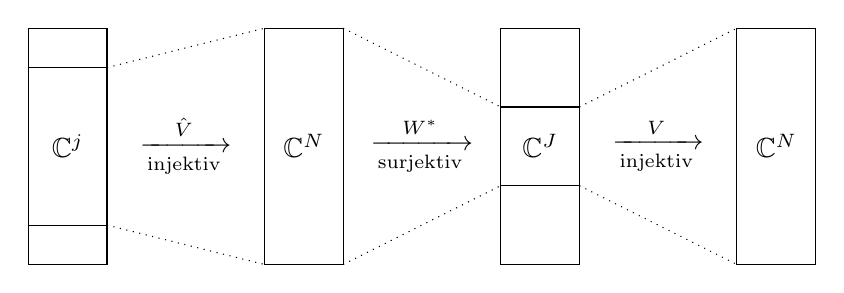
\begin{tikzpicture}[scale = 0.5]

        \draw (0,  0) rectangle (2,  6);
        \draw (6,  0) rectangle (8,  6);
        \draw (12, 0) rectangle (14, 6);
        \draw (18, 0) rectangle (20, 6);

        \draw (0, 1) -- (2, 1);
        \draw (0, 5) -- (2, 5);

        \draw [dotted] (2, 1) -- (6, 0);
        \draw [dotted] (2, 5) -- (6, 6);

        \draw [dotted] (8, 0) -- (12, 2);
        \draw [dotted] (8, 6) -- (12, 4);

        \draw (12, 2) -- (14, 2);
        \draw (12, 4) -- (14, 4);

        \draw [dotted] (14, 2) -- (18, 0);
        \draw [dotted] (14, 4) -- (18, 6);

        \draw (1,  3) node {$\C^j$};
        \draw (4,  3) node {$\xrightarrow[\text{injektiv}]{\hat V}$};
        \draw (7,  3) node {$\C^N$};
        \draw (10, 3) node {$\xrightarrow[\text{surjektiv}]{W^\ast}$};
        \draw (13, 3) node {$\C^J$};
        \draw (16, 3) node {$\xrightarrow[\text{injektiv}]{V}$};
        \draw (19, 3) node {$\C^N$};

    \end{tikzpicture}
    \caption{}
    \label{fig:rang_1}
\end{figure}

Matrizen haben genau dann denselben Rang, wenn sie äquivalent sind.

\begin{align*}
    \begin{pmatrix}
        \diag(\sigma_1, \dots, \sigma_J, \dots, \sigma_j) \\
        0_{(N - j) \times j}
    \end{pmatrix}
    =
    \Sigma
    \equiv
    \tilde V \Sigma \tilde W^\ast
    =
    A_0
    \equiv
    \begin{pmatrix}
        I_J \enspace 0_{J \times (j - J)} \\ 0_{(N - J) \times j}
    \end{pmatrix}
\end{align*}

Damit verschwinden die letzten Singulärwerte $\sigma_{J+1} = \cdots = \sigma_j = 0$.
Somit können wir statt der vollen Singulärwert-Zerlegung (indiziert mit \Quote{full}) eine reduzierte (indiziert mit \Quote{reduced}) verwenden.

\begin{align*}
    A_0
    =
    \tilde V_\mathrm{full} \Sigma_\mathrm{full} \tilde W_\mathrm{full}^\ast
    =
    \begin{pmatrix}
        \tilde V_\mathrm{reduced} & \ast
    \end{pmatrix}
    \begin{pmatrix}
        \Sigma_\mathrm{reduced} & 0_{J \times (j - J)}       \\
        0_{(N - J) \times J}    & 0_{(N - J) \times (j - J)}
    \end{pmatrix}
    \begin{pmatrix}
        \tilde W_\mathrm{reduced}^\ast \\ \ast
    \end{pmatrix}
    =
    \tilde V_\mathrm{reduced} \Sigma_\mathrm{reduced} \tilde W_\mathrm{reduced}^\ast
\end{align*}

Die $\tilde V_\mathrm{full}$ und $\tilde W_\mathrm{full}$ sind ja unitär, d.h. ihre Adjungierten waren ihre Inversen.

\begin{align*}
    \implies
    I_{N \times N}
    =
    \tilde V_\mathrm{full}^\ast \tilde V_\mathrm{full}
    =
    \begin{pmatrix}
        \tilde V_\mathrm{reduced}^\ast \\ \ast
    \end{pmatrix}
    \begin{pmatrix}
        \tilde V_\mathrm{reduced} & \ast
    \end{pmatrix}
    =
    \begin{pmatrix}
        \tilde V_\mathrm{reduced}^\ast \tilde V_\mathrm{reduced} & \ast \\
        \ast                                                     & \ast
    \end{pmatrix}
\end{align*}

Eine analoge Rechnung kann man, mit $j$ anstelle von $N$, für $\tilde W_\mathrm{reduced}$ machen.
Insgesamt erhalten wir also folgende Tatsachen über unsere reduzierte Singulärwert-Zerlegung.
Wir vereinbaren, ab sofort nur noch die reduzierte Singulärwert-Zerlegung zu verwenden und den Index wegzulassen.

\begin{align} \label{eq:singulärwert_zerlegung}
    \tilde V^\ast \tilde V
    =
    \tilde W^\ast \tilde W
    =
    I_{J \times J},
    \quad
    \Sigma = \diag(\sigma_1, \dots, \sigma_J),
    \quad
    A_0 = \tilde V \Sigma \tilde W^\ast
\end{align}

$\tilde V$ hat, als Teil-Matrix einer unitären, vollen Spaltenrang $J$ hat.
$\tilde V^\ast$ hat also vollen Zeilenrang $J$.
Abbildung \ref{fig:rang_2} illustriert, dass $S := \tilde V^\ast V \in \C^{J \times J}$ genau $J$ linear unabhängige Spalten hat, also $S \in \GL_J(\C)$.

\begin{figure}[!ht]
    \centering
    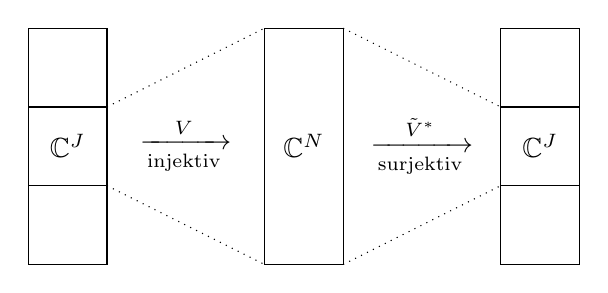
\begin{tikzpicture}[scale = 0.5]

        \draw (0,  0) rectangle (2,  6);
        \draw (6,  0) rectangle (8,  6);
        \draw (12, 0) rectangle (14, 6);

        \draw (0, 2) -- (2, 2);
        \draw (0, 4) -- (2, 4);

        \draw [dotted] (2, 2) -- (6, 0);
        \draw [dotted] (2, 4) -- (6, 6);

        \draw [dotted] (8, 0) -- (12, 2);
        \draw [dotted] (8, 6) -- (12, 4);

        \draw (12, 2) -- (14, 2);
        \draw (12, 4) -- (14, 4);

        \draw (1,  3) node {$\C^J$};
        \draw (4,  3) node {$\xrightarrow[\text{injektiv}]{V}$};
        \draw (7,  3) node {$\C^N$};
        \draw (10, 3) node {$\xrightarrow[\text{surjektiv}]{\tilde V^\ast}$};
        \draw (13, 3) node {$\C^J$};

    \end{tikzpicture}
    \caption{}
    \label{fig:rang_2}
\end{figure}

In den folgenden Gleichungsketten wird bei \Quote{!} die jeweils vorgerige eingesetzt.

\begin{align*}
    & \implies
    \Sigma \tilde W^\ast
    \stackrel
    {
        \eqref{eq:singulärwert_zerlegung}
    }{=}
    \tilde V^\ast \tilde V \Sigma \tilde W^\ast
    \stackrel
    {
        \eqref{eq:singulärwert_zerlegung}
    }{=}
    \tilde V^\ast A_0
    \stackrel
    {
        \eqref{eq:integral_matrizen_resultat}
    }{=}
    \tilde V^\ast V W^\ast \hat V
    =
    S W^\ast \hat V \\
    & \implies
    A_1
    \stackrel
    {
        \eqref{eq:integral_matrizen_resultat}
    }{=}
    V D W^\ast \hat V
    \stackrel{!}{=}
    V D S^{-1} \Sigma \tilde W^\ast \\
    & \implies
    \tilde V^\ast A_1 \tilde W \Sigma^{-1}
    \stackrel{!}{=}
    \tilde V^\ast V D S^{-1} \Sigma \tilde W^\ast \tilde W \Sigma^{-1}
    =
    S D S^{-1}
    \approx
    D
\end{align*}

Somit ist die Diagonalmatrix $D$, welche ja die gesuchten Eigenwerte enthält, ähnlich zur Matrix $\tilde V^\ast A_1 \tilde W \Sigma^{-1}$.
Ähnliche Matrizen haben dieselben Eigenwerte.

\subsection*{Zusammenfassung}

Wir haben insgesamt den folgenden Algorithmus \ref{alg:integral_methode_zusammenfassung} gefunden.

\begin{algorithm}[H]
	\label{alg:integral_methode_zusammenfassung}
	\caption{Integral-Methode}
    \begin{algorithmic}[1]
        \Procedure{Integral-Methode Zusammanfassung}{}
            \State Berechne $A_0, A_1 \in \C^{N \times j}$ (z.B. mit LU-Zerlegung);
            \State Berechne und reduziere eine Singulärwert-Zerlegung $A_0 = \tilde V \Sigma \tilde W^\ast$ auf $J$ Singulärwerte;
            \State Berechne Eigenwerte $\lambda_1, \dots, \lambda_k$ der Matrix $\tilde V A_1 \tilde W \Sigma^{-1}$ (z.B. mit QR-Verfahren);
            \State \Return $\lambda_1, \dots, \lambda_k$
		\EndProcedure
	\end{algorithmic}
\end{algorithm}

% -------------------------------------------------------------------------------- %

\begin{exercise}

Zeigen Sie, dass für alle $n \geq 1$ gilt:
$(n! + 1, (n+1)! + 1) = 1$.

\end{exercise}

% -------------------------------------------------------------------------------- %

\begin{solution}

Um eine erste Idee zur Lösung zu erhalten, betrachten wir
zuerst einige Beispiele für kleine $n$:

\begin{align*}
  n &= 1: (2, 3) = 1 \\
  n &= 2: (3, 7) = 1 \\
  n &= 3: (7, 25) = (7, 5 \cdot 5) = 1 \\
  n &= 4: (25, 121) = (5 \cdot 5, 11 \cdot 11) = 1 \\
  n &= 5: (121, 721) = (11 \cdot 11, 7 \cdot 103) = 1
\end{align*}

Sei nun angenommen, dass $d := (n! + 1, (n+1)! + 1)  > 1$.

Da $(n+1)! + 1 - (n! + 1) = n!\cdot n$ folgt $d | n! \cdot n$.

Nun unterscheiden wir zwei Fälle:

\begin{itemize}
  \item[$(d,n) = 1$:] In dem Fall erhalten wir direkt $d | n!$ und 
  mit $d | (n! + 1 - n!) = 1$ einen Widerspruch!
  \item[$(d,n) > 1$:] In diesem Fall folgt aus $(d,n) | d$ und $d | n! + 1$, 
  sowie $(d,n) | n$ und $n | n!$,
  dass $(d,n) | (n! + 1 - n!) = 1$ mit Widerspruch zu $(d,n) > 1$!
\end{itemize}

\end{solution}

% -------------------------------------------------------------------------------- %

% -------------------------------------------------------------------------------- %

\begin{exercise}[Legendre]

Zeigen Sie, dass die Zahl $n!$ den Primfaktor $p$ genau

\begin{align*}
  \sum_{k \geq 1} \left\lfloor \frac{n}{p^k}\right\rfloor
\end{align*}
Mal enthält.
\end{exercise}

% -------------------------------------------------------------------------------- %

\begin{solution}

Die Zahl $n!$ enthält den Primfaktor $p$ genau $\sum_{i=1}^n \nu_p(i)$ Mal.
Die Zahlen bis $n$, welche den Primfaktor $p$ mindestens einmal enthalten sind genau
$p,2p,\dots,\left\lfloor \frac{n}{p}\right\rfloor p$.
Ebenso gibt es genau $\left\lfloor \frac{n}{p^k}\right\rfloor$ Zahlen bis $n$,
welche den Primfaktor $p$ mindestens $k$ Mal enthalten. \\
Damit erhalten wir mit $\sum_{k \geq 1} \left\lfloor \frac{n}{p^k}\right\rfloor$
genau die Anzahl, wie oft der Primfaktor $p$ in $n!$ enthalten ist.

\end{solution}

% -------------------------------------------------------------------------------- %

\begin{exercise}

Sei $X$ ein topologischer Vektorraum.
Eine Menge $B \subseteq X$ heißt beschränkt, falls es zu jeder Nullumgebung $U$ ein positive Zahl $\lambda_U$ gibt, sodass $B \subseteq \lambda_U U$.
Zeige, dass jede kompakte Teilmenge von $X$ beschränkt ist. Zeige, dass jeder lineare Teilraum $Y \neq \Bbraces{0}$ von $X$ unbeschränkt ist.

\end{exercise}

\begin{solution}

Trivial!

\end{solution}

\begin{exercise}

Sei $X$ ein topologischer Vektorraum und $B \subseteq X$.
Zeige, dass die folgenden Aussagen äquivalent sind:

\begin{enumerate}[label = (\roman*)]
  \item $B$ ist beschränkt.
  \item Zu jeder Nullumgebung $U$ gibt es eine Zahl $\mu_U > 0$, sodass $B \subseteq \lambda U$ für alle $\lambda > \mu_U$.
  \item Für jede Folge $(x_n)_{n \in \N}$ von Elementen von $B$ und jede Folge $(\alpha_n)_{n \in \N}$ komplexer Zahlen mit $\lim_{n \to \infty} \alpha_n = 0$ gilt $\lim_{n \to \infty} \alpha_n x_n = 0$.
\end{enumerate}

\end{exercise}

\begin{solution}

\Quote{(i) $\Rightarrow$ (ii)}:
Seien $W, U \in \mathfrak{U}(0)$, mit $W \subseteq U$ kreisförmig.
Nachdem $B$ beschränkt ist, $\Exists \mu_U > 0: \Forall \lambda > \mu_U:$

\begin{align*}
  B
  \subseteq
  \mu_U W
  \stackrel{!}{\subseteq}
  \lambda W
  \subseteq
  \lambda U.
\end{align*}

Dabei gilt \Quote{!}, weil $|\frac{\mu_u}{\lambda}| \leq 1$ und somit $\frac{\mu_u}{\lambda} W \subseteq W$, da $W$ kreisförmig ist. \\

\Quote{(ii) $\Rightarrow$ (i)}:
Trivial! \\

\Quote{(i) $\Rightarrow$ (iii)}:
Sei $U \in \mathfrak{U}(0)$ kreisförmig, und $(x_n) \in B$.
Weil $B$ beschränkt ist, $\Exists \lambda > 0: (x_n) \in B \subseteq \lambda U$.
Wenn nun $(\alpha_n) \in \C$, mit $\alpha_n \to 0$, dann gilt für fast alle $n \in \N:$

\begin{align*}
  |\alpha_n| \leq \frac{1}{\lambda}
  \Rightarrow
  \frac{x_n}{\lambda} \in U,
  |\alpha_n \lambda| \leq 1
  \Rightarrow
  \alpha_n x_n \in U.
\end{align*}

\Quote{(iii) $\Rightarrow$ (i)}:
Angenommen, $\Exists U \in \mathfrak{U}(0): \Forall \lambda > 0: B \not \subseteq \lambda U$, d.h. $\Exists x_\lambda \in B: x_\lambda \notin \lambda U$.
Sei nun $(\alpha_n) \in \R^+: \alpha_n \to 0$ und definiere $\lambda_n := \frac{1}{\alpha_n}$.
Weil $B$ ja nicht beschränkt ist, muss $\Forall n \in \N: \Exists x_n \in B:$

\begin{align*}
  x_n \notin \lambda_n U
  \Rightarrow
  \alpha_n x_n \notin U.
\end{align*}

Somit $\Exists (x_n) \in B, \Exists (\alpha_n) \in \C: \alpha_n \to 0, \alpha_n x_n \not \to 0$, d.h. $\Exists U \in \mathfrak{U}(0): \Forall N \in \N: \Exists n \geq N: \alpha_n x_n \notin U$.

\end{solution}


\end{document}
